\chapter{线性映射及其矩阵表示}

\section{Overview}
\begin{figure}[h]
	\centering
	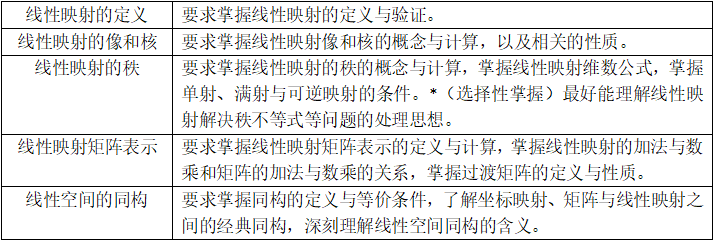
\includegraphics[scale=0.58]{2.png}
\end{figure}

\section{线性映射的定义}
\subsection{线性映射的定义}
\begin{definition}
	从线性空间$V_1(\mathbf{F})$到$V_2(\mathbf{F})$的一个映射$\sigma$是线性的,
	如果$\forall \alpha,\beta \in V_1$和$\forall \lambda,\mu \in \mathbf{F}$都有
	\begin{equation}
		\sigma(\lambda\alpha+\mu\beta)=\lambda\sigma(\alpha)+\mu\sigma(\beta).
	\end{equation}
	
	从线性空间$V$到自身的线性映射$\sigma$也叫作$V$上的线性变换,
	从线性空间$V(\mathbf{F})$到域$\mathbf{F}$的线性映射$f$叫作$V$上的线性函数(线性形式).
\end{definition}
实际上,上述定义式(1)可以分拆为以下(2)(3)式:
\begin{equation}
	\sigma(\alpha+\beta)=\sigma(\alpha)+\sigma(\beta)
\end{equation}
\begin{equation}
	\sigma(\lambda\alpha)=\lambda\sigma(\alpha)
\end{equation}
其中(2)称为加性,(3)称为齐次性.

根据定义,我们容易知道熟悉的过原点的直线(一次函数)是线性映射,而不过原点的直线不代表线性映射。

特别注意:根据定义,线性映射一定将出发空间的零元映射到到达空间的零元,
这是一个映射为线性映射的必要条件。
\subsection{线性映射的基本运算}
本节介绍线性映射的加法、数乘的定义,并介绍线性映射乘法(即复合)和逆运算。

我们需要首先说明一个记号,我们把线性空间$V_1(\mathbf{F})$到$V_2(\mathbf{F})$的所有线性映射组成的集合记作$L(V_1,V_2)$.
我们希望在这个集合上定义线性空间,于是需要定义其中元素(线性映射)的加法和数乘运算:
\begin{definition}
	设$\sigma,\ \tau\in L(V_1,V_2)$,规定$\sigma$与$\tau$之和及$\lambda$与
	$\sigma$的数乘$\lambda\sigma$分别为
	\begin{equation}
		(\sigma+\tau)(\alpha)=\sigma(\alpha)+\tau(\alpha),\ \forall\alpha\in V_1
	\end{equation}
	\begin{equation}
		(\lambda\sigma)(\alpha)=\lambda(\sigma(\alpha)),\ \forall\alpha\in V_1
	\end{equation}
\end{definition}
\begin{example}
	证明:$L(V_1,V_2)$与上述定义的线性映射加法和数乘构成域$\mathbf{F}$上的线性空间.
\end{example}
下面讨论线性映射的复合。设$\sigma \in L(V_1,V_2),\ \tau \in L(V_2,V_3)$,则$\tau\sigma$是$L(V_1,V_3)$
中的元素,且$\tau\sigma(\alpha)=\tau(\sigma(\alpha)),\ \forall \alpha \in V_1$.
\begin{example}
	证明:上述定义的映射$\tau\sigma$是线性映射.
\end{example}
注意:在上述定义中一定注意$\sigma$和$\tau$的顺序,我们需要先使用$\sigma$将$V_1$中的元素映射到
$V_2$,然后再用外层的$\tau$映射到$V_3$。

下面定义逆映射。如果可逆映射$\sigma:V_1 \to V_2$的逆映射为$\sigma^{-1}$,则$\sigma^{-1}\sigma=I_{V_1}$且
$\sigma\sigma^{-1}=I_{V_2}$。其中$I_{V}$的含义为$V$上的恒等映射,即$I_V(\alpha)=\alpha,\ \forall \alpha \in V$。
\begin{example}
	证明:上述定义的逆映射$\sigma^{-1}$为线性映射.
\end{example}
\subsection{线性映射举例}
本节内容希望各位同学按照教材3.1节例1-9了解常见的线性映射,了解一定的几何意义(虽然不会直接考察,但是对理解有帮助)。
其中例1、7、8、9希望同学们当做练习,例2中旋转变换的矩阵表示的求幂在矩阵计算专题中有提及,
例3镜面变换本是重点,但今年不要求内积空间,例6投影变换将在幂等矩阵中我们会再次提及。
\subsection{线性映射的确定}
有限维空间上的线性映射被基上的像唯一确定,即
\begin{theorem}
	已知线性映射$\sigma,\tau\in L(V_1,V_2)$,且有$V_1$的基$B=\{\alpha_1,\alpha_2,\cdots,\alpha_n\}$,
	若$\sigma(\alpha_i)=\tau(\alpha_i),\ \forall \alpha_i \in B$,则有$\sigma=\tau$.
\end{theorem}
即映射在一组基上的像确定了,则映射是唯一的。这一证明是容易的,希望同学自行尝试。
进一步地,我们有如下定理:
\begin{theorem}
	设$B=\{\alpha_1,\alpha_2,\cdots,\alpha_n\}$是$V_1(\mathrm{T})$的基,$S=\{\beta_1,\beta_2,\cdots,\beta_n\}$
	是$V_2$中任意$n$个向量,则存在唯一的$\sigma\in L(V_1,V_2)$使得$\sigma(\alpha_i)=\beta_i,\ i=1,2,\cdots,n$.
\end{theorem}
这一定理即教材定理3.6,希望同学们自己先尝试自己证明,只需先定义映射然后证明其线性性即可,唯一性在上一个定理中已经说明。
\subsection{习题}
\centerline{\heiti A组}
\begin{enumerate}
	\item 写出下列映射的出发空间和到达空间,并判断其是否为线性映射:
	
	(1)$\sigma(x_1,x_2)=(x_1-x_2,x_1,x_1+x_2)$;

	(2)$\sigma(x_1,x_2)=(x_1x_2,x_1+x_2)$;

	(3)$\sigma(p(x))=p(x+1)-p(x),\ \forall p(x) \in \mathbf{R}[x]_n$;

	(4)$\sigma(p(x))=p(a),\ \forall p(x)$,其中$a$为常数;

	(5)$\sigma(\xi)=2\xi+\xi_0$,其中$\xi$是线性空间$V$中的一个固定向量.
	\item 设$\sigma,\tau \in L(V,V)$且$\sigma^2=\sigma$,$\tau^2=\tau$,证明:
	
	(1)$\sigma^k=\sigma$(幂等变换);

	(2)若$(\sigma+\tau)^2=\sigma+\tau$,则$\sigma\tau=\theta$(零变换);

	(3)设$\sigma\tau=\tau\sigma$,则$(\sigma+\tau-\sigma\tau)^2=\sigma+\tau-\sigma\tau$.
	\item 是否存在$\mathbf{R}^3$到$\mathbf{R}^2$的线性映射$\sigma$使得$\sigma(1,-1,1)=(1,0)$,
	$\sigma(1,1,1)=(0,1)$.
\end{enumerate}
\centerline{\heiti B组}
\begin{enumerate}
	\item 已知
	$$\alpha_1=(1,-1),\alpha_2=(2,-1),\alpha_3=(-3,2);$$
	$$\beta_1=(1,0),\beta_2=(0,1),\beta_3=(1,1).$$
	是否存在$\sigma\in L(\mathbf{R}^2,\mathbf{R}^2)$,使得$\sigma(\alpha_i)=\beta_i(i=1,2,3)$.
	\item 设$\{\alpha_1,\alpha_2\}$是线性空间$V(\mathbf{F})$的一组基,$x_1\alpha_1+x_2\alpha_2 \in V$,
	定义$T(x_1\alpha_1+x_2\alpha_2)=r_1x_1\alpha_1+r_2x_2\alpha_2$,其中$r_1,r_2$是域$F$中的两个常数,
	证明:$T$是$V$上的一个线性变换,当$V=\mathbf{R}^2$时,说明$T$的几何意义.
	\item 已知$\mathbf{R}$上的线性变换$\sigma(x_1,x_2)=(x_1-x_2,x_1+x_2)$,$\tau(x_1,x_2)=(x_1-x_2,x_1-x_2)$.
	
	(1)求$\sigma^2(x_1,x_2)$;

	(2)$\sigma$是否可逆?如可逆,求$\sigma^{-1}(x_1,x_2)$;

	(3)求$\xi\in L(\mathbf{R}^2,\mathbf{R}^2)$,使得$\xi\tau=\theta$(零变换).
	\item 设$A,B,C,D \in \mathbf{F}^{n \times n}$,若
	$$T:X \to AXB+CX+XD,\ \forall X \in \mathbf{F}^{n \times n}.$$
	证明:

	(1)$T$为$\mathbf{F}^{n \times n}$上的线性变换;

	(2)当$C=D=0$时,$T$可逆的充要条件是$|AB| \neq 0$.
\end{enumerate}
\centerline{\heiti C组}
\begin{enumerate}
	\item 设 $V(\mathbf{F})$ 是一个 $n$ 维线性空间,$\sigma \in L(V,\ V)$,证明:

	(1)在 $\mathbf{F}[x]$ 中有一个次数不高于 $n^2$ 的多项式 $p(x)$ 使 $p(\sigma)=0$;
	
	(2)$\sigma$ 可逆$\iff$有一常数项不为 $0$ 的多项式 $p(x)$ 使 $p(\sigma)=0$。
\end{enumerate}

\section{线性映射的像、核与秩}
\subsection{线性映射的像和核的定义}
\begin{definition}
	设$\sigma$是线性空间$V_1(\mathbf{F})$到$V_2(\mathbf{F})$的线性映射,$V_1$的所有元素
	在$\sigma$下的像组成的集合
	$$\sigma(V_1)=\{\beta\ |\ \beta=\sigma(\alpha),\ \alpha \in V_1\}$$
	称为$\sigma$的像(或值域),记作$\textup{Im }\sigma$,$V_2$的零元$0_2$在$\sigma$下的完全原像
	$$\sigma^{-1}(0_2)=\{\alpha\ |\ \sigma(\alpha)=0_2,\ \alpha \in V_!\}$$
	称为$\sigma$的核,记作$\ker \sigma$.
\end{definition}
注意核的定义中$0_2$代表$V_2$中的零元,实际上下标也可以省略。

注意,线性映射的像和核分别是$V_2$和$V_1$的子空间。同样地,若$W_1$和$W_2$分别是$V_1$和$V_2$的
子空间,则$\sigma(W_1)$和$\sigma^{-1}(W_2)$也分别是$V_2$和$V_1$的子空间。以上命题的证明很简单,各位可以自行尝试。

下面是一种经典题型,即已知线性映射求线性映射的像和核,注意方法如下:

1. 像空间$\textup{Im }\sigma=\sigma(V_1)=L(\sigma(\alpha_1),\sigma(\alpha_2),\cdots,\sigma(\alpha_n))$,即线性映射在
一组基下的像的线性扩张,解答写出极大线性无关组然后扩张即可;

2. 核空间直接令$\sigma(\alpha)=0$,利用解线性方程组得到解$\alpha$,结果的线性扩张即为核空间。
\begin{example}
	已知$\mathbf{R}^3$到$\mathbf{R}^2$的映射$\sigma$为$\sigma(x_1,x_2,x_3)=(x_1+x_2,x_2-x_3)$,
	求$\sigma$的像和核.
\end{example}
\subsection{线性映射的秩的定义}
我们已知$\textup{Im }\sigma=\sigma(V_1)=L(\sigma(\alpha_1),\sigma(\alpha_2),\cdots,\sigma(\alpha_n))$,
我们基于此定义线性映射的秩:
\begin{definition}
	设$\sigma\in L(V_1,V_2)$,如果$\sigma(V_1)$是$V_2$的有限维子空间,则
	$\sigma(V_1)$的维数称为$\sigma$的秩,记作$r(\sigma)$,即$r(\sigma)=\dim \sigma(V_1)$.
\end{definition}
简单理解即线性映射的秩即为线性映射像空间的维数。
\subsection{线性映射基本定理(维数公式)}
这一定理是本学期最重要的定理之一,因其重要性也被冠以线性映射基本定理(有线维线性空间)的名号:
\begin{theorem}
	设$\sigma \in L(V_1,V_2)$,若$\dim V_1=n$,则
	$$r(\sigma)+\dim\ker\sigma=n.$$
\end{theorem}
这一定理的证明方式希望大家熟练掌握,下面是一个思想上类似的例子:
\begin{example}
	设$\sigma$为有限维线性空间$V$上的线性变换,$W$是$V$的子空间,证明:
	$$\dim\sigma(W)+\dim(\sigma^{-1}(0) \cap W)=\dim W.$$
\end{example}
基于线性映射基本定理,我们可以得到如下定理:
\begin{theorem}
	对$\sigma \in L(V_1,V_2)$且$\dim V_1=\dim V_2=n$,我们有
	$\ker\sigma=\{0\}\iff \sigma$为单射$\iff \sigma$为满射$\iff \sigma$为双射(可逆)$\iff r(\sigma)=n$(满秩).
\end{theorem}
显然这一定理前提适用于一切有限维空间上的线性变换。我们需要注意的是,上述第一个等价式不是基于线性映射基本定理得到的,
是教材定理3.1的内容,证明较为容易,建议先自己尝试证明。

线性映射基本定理还隐藏着一个结论,即不可能存在从低维空间到高维空间的满射(反证法代入维数公式即可,当然也可以利用线性相关性证明)。
\subsection{线性映射的像和核的进一步讨论}
\textbf{注:本节内容如果时间不够可以快速略过,只需大致了解重要原则以及结论即可。}

关于线性变换的像和核有很多的包含关系或等式等结论,实际上很多问题都来源于线性映射基本定理及其推论,本节我们主要探讨这一话题。

我们首先说明几个重要的原则:

1. 解决此类问题大多需要综合利用维数公式及其推论,需要讲题给条件转化为合适的等价表述然后解决;

2. 注意集合相等的证明方式,实际上就是两个集合互相包含。实际上很多时候一边的包含是显然的,只需证明另一边;

3. 时刻注意线性映射的像和核的定义,线性空间的交、和与直和的概念,例如看到像需要想到其存在原像,看到和与直和要想到将向量分拆等。

接下来我们看一些经典的结论(已知$V$为有限维线性空间,$\sigma\in L(V,V)$),有余力的同学可以思考其证明,其中结论1最为常见:

1. 若$\sigma$为幂等变换(即$\sigma^2=\sigma$)有$V=\ker\sigma\oplus\textup{Im }\sigma$;

2. $r(\sigma^2)=r(\sigma) \iff V=\ker\sigma\oplus\textup{Im }\sigma$;

3. $\ker\sigma=\ker\sigma^2 \iff \ker\sigma \cap \textup{Im }\sigma=\{0\} \iff \textup{Im }\sigma=\textup{Im }\sigma^2 \iff V=\ker\sigma\oplus \textup{Im }\sigma$;

4. $\ker\sigma \subseteq \ker\sigma^2 \subseteq \ker\sigma^3 \subseteq \cdots$;

5. $\textup{Im }\sigma \supseteq \textup{Im }\sigma^2 \supseteq \textup{Im }\sigma^3 \supseteq \cdots$;

6. 存在正整数$m$使得对任意的$n>m$都有$\ker\sigma^n=\ker\sigma^m$,$\textup{Im }\sigma^n=\textup{Im }\sigma^m$;

7. 存在正整数$m$使得$V=\textup{Im }\sigma^m+\ker\sigma^m$;

8. $\dim(\ker\sigma+\textup{Im }\sigma) \ge \cfrac{n}{2}$,等号成立充要条件为$\ker\sigma=\textup{Im }\sigma$.
\subsection{习题}
\centerline{\heiti A组}
\begin{enumerate}
	\item 是否存在$\mathbf{R}^2$到$\mathbf{R}^3$的线性映射$\sigma$使得$\sigma(3,2)=(1,0,0)$,$\sigma(1,5)=(1,1,0)$,$\sigma(-1,4)=(1,1,1)$.
	\item 求$\sigma(x_1,x_2,\cdots,x_n)=(x_1,0,\cdots,0)$的像、核与秩.
\end{enumerate}
\centerline{\heiti B组}
\begin{enumerate}
	\item 已知$\mathbf{R}^3$上的两个线性变换$\sigma,\tau$为:
	$$\sigma(x_1,x_2,x_3)=(x_3,0,0),$$
	$$\tau(x_1,x_2,x_3)=(x_1+x_2+x_3,x_1-x_2,0).$$
	(1)求$r(\sigma)$,$r(\tau)$,$\textup{Im }\sigma$,$\ker\sigma$;

	(2)求$r(\tau\sigma)$,$r(\sigma\tau)$,$r(\sigma+\tau)$;

	(3)求$\textup{Im }\tau+\ker\tau$.
	\item 设$\sigma(p(x))=p'(x)$(求导),$\forall p(x) \in \mathbf{R}[x]_n$.
	
	(1)证明:$\sigma$是$\mathbf{R}[x]_n$上的线性变换;

	(2)求$\sigma$的值域和$r(\sigma)$,说明$\sigma$是否可逆;

	(3)求$\sigma$的核及其维数;

	(4)求$r(\sigma)+\dim\ker\sigma$,问:$\mathbf{R}[x]_n=\ker\sigma+\textup{Im }\sigma$是否成立.
	\item 设$V$为有限维线性空间,$T\in L(V,V)$且$T$不是恒等变换也不是零变换,问:下列情况是否可能发生,
	如果可能请举例,不可能请说明理由.

	(1)$\textup{Im }T \cap \ker T = \{0\}$;

	(2)$\textup{Im }T \subset \ker T$;

	(3)$\ker T = \textup{Im }T$;

	(4)$\ker T \subset \textup{Im }T$.
	\item 若$\sigma_1,\sigma_2\in L(V,V)$,判断下列说法是否正确,正确请给出证明,反之给出反例:
	
	(1)由$r(\sigma)+\dim\ker\sigma=n$可知$V=\ker\sigma+\textup{Im }\sigma$;

	(2)若有$\textup{Im }T \cap \ker T = \{0\}$,则$V=\ker\sigma+\textup{Im }\sigma$成立;

	(3)因为$\forall \alpha \in V$有$(\sigma_1+\sigma_2)(\alpha)=\sigma_1(\alpha)+\sigma_2(\alpha)$,
	所以$(\sigma_1+\sigma_2)(V)=\sigma_1(V)+\sigma_2(V)$;

	(4)$(I-\sigma)(V)+\sigma(V)=V$($I$为恒等映射).
	\item 已知$V$为有限维线性空间,$\sigma\in L(V,V)$,且$\ker\sigma=\textup{Im }\sigma$,证明:
	
	(1)$n$为偶数;

	(2)存在$V$的一组基$\alpha_1,\cdots,\alpha_n$使得
	$$\sigma(\alpha_1,\cdots,\alpha_n)=(\alpha_1,\cdots,\alpha_n)\begin{pmatrix}
		0 & E_{\frac{n}{2}} \\ 0 & 0
	\end{pmatrix}.$$
\end{enumerate}
\centerline{\heiti C组}
\begin{enumerate}
	\item 设$V$是一个$n$维线性空间,$V=W_1\oplus W_2$,$\sigma\in L(V,V)$,证明:$\sigma$可逆$\iff V=\sigma(W_1)+\sigma(W_2)$.
	\item 设$V_1,V_2,V_3$分别为$m,n,s$维线性空间,$\sigma\in L(V_1,V_2),\tau\in L(V_2,V_3)$,则
	$$r(\sigma)+r(\tau)-n \le r(\tau\sigma) \le \min(r(\sigma),r(\tau)).$$
	\item 设$V_1$是有线维线性空间,$\sigma,\tau\in L(V_1,V_2)$,则
	$$r(\sigma+\tau) \le r(\sigma)+r(\tau).$$
	
	事实上前两题的结论在下一章节矩阵的秩中都会涉及,此处有兴趣的同学可以尝试从线性映射的角度理解这两个秩不等式.
	由于这是教材中小字部分内容,一般而言不在考察范围,如果出现且无法找到合适方式,可以考虑化为矩阵进行证明.
	\item 设$\sigma\in L(V,V)$,$\dim V_1=n$,且$\sigma^2=\sigma$,$I$是$V$上的恒等变换,证明:
	
	(1)$(I-\sigma)(V) \in \ker\sigma$;

	(2)$r(I-\sigma)+r(\sigma)=n$.
	\item 已知$V$为有限维线性空间,$\sigma\in L(V,V)$,且$\sigma^2=\theta$(零映射),证明:
	
	(1)$\sigma$的像空间维数不超过$\cfrac{n}{2}$;

	(2)设$A$是$\sigma$在某组基下的矩阵,则方程组$AX=0$的基础解系至少有$\cfrac{n}{2}$个解.
\end{enumerate}

\section{线性映射矩阵表示}
\subsection{一个最基本的定义}
\begin{definition}
	设$B_1=\{\epsilon_1,\epsilon_2,\dots,\epsilon_n\}$是$V_1(F)$的基,$B_2=\{\alpha_1,\alpha_2,\cdots,\alpha_m\}$是$V_2(F)$的基,
	则线性映射$\sigma \in L(V_1,V_2)$被它作用于基$B_1$的像
	$$\sigma(B_1)=\{\sigma(\epsilon_1),\sigma(\epsilon_2),\dots,\sigma(\epsilon_n)\}$$
	所唯一确定,而$\sigma(B_1)$是$V_2$的一个子集,于是
	$$\begin{cases}
		\sigma(\epsilon_1)=a_{11}\alpha_1+a_{21}\alpha_2+\cdots+a_{m1}\alpha_m \\
		\sigma(\epsilon_2)=a_{12}\alpha_1+a_{22}\alpha_2+\cdots+a_{m2}\alpha_m \\
		\cdots \\
		\sigma(\epsilon_n)=a_{1n}\alpha_1+a_{2n}\alpha_2+\cdots+a_{mn}\alpha_m
	\end{cases}.$$
	我们将$\sigma(B_1)=\{\sigma(\epsilon_1),\sigma(\epsilon_2),\dots,\sigma(\epsilon_n)\}$
	关于基$B_2$的坐标排列成矩阵$M(\sigma)$,即
	$$M(\sigma)=\begin{pmatrix}
		a_{11} & a_{12} & \cdots & a_{1n} \\
		a_{21} & a_{22} & \cdots & a_{2n} \\
		\cdots & \cdots &        & \cdots \\
		a_{m1} & a_{m2} & \cdots & a_{mn}
	\end{pmatrix}.$$
\end{definition}
更通俗来说,线性映射矩阵表示就是将线性映射在一组基上的像在另一组基下的坐标按列排列的结果。

之后我们会经常看见两种记号,即$(\sigma(\epsilon_1),\sigma(\epsilon_2),\dots,\sigma(\epsilon_n))$ 
和$\sigma(\epsilon_1,\epsilon_2,\dots,\epsilon_n)$。实际上是等价的,等价原因是
$(\sigma(\epsilon_1),\sigma(\epsilon_2),\dots,\sigma(\epsilon_n))A=(\sigma(\epsilon_1,\epsilon_2,\dots,\epsilon_n))A=\sigma((\epsilon_1,\epsilon_2,\dots,\epsilon_n)A)$成立,
这一性质在之后会有运用,证明并不复杂,可以自行尝试或参考我的矩阵辅学授课。

除此之外,我们还应当强调以下结论,在我们后续研究线性方程组解的相关性质时是常用的:
\begin{theorem}
	线性映射是单射当且仅当其矩阵表示为列满秩矩阵,线性映射是满射当且仅当其矩阵表示为行满秩矩阵.
\end{theorem}
这一结论的证明比较基本,希望大家能透过这一个结论看到列满秩矩阵与行满秩矩阵更本质的特征。
\subsection{一组简单的例子}
\begin{example}
	已知$\sigma \in L(\mathbf{R}^3,\mathbf{R}^3)$且$\sigma(x_1,x_2,x_3)=(x_1+x_2,x_1-x_3, x_2)$
	
	\textup{(1)}求$\sigma$的像空间和核空间;

	\textup{(2)}求$\sigma$关于$\mathbf{R}^3$自然基的矩阵.
\end{example}

\begin{example}
	设$A=\begin{pmatrix}1 & 0 & 2 \\ -1 & 2 & 1 \\ 1 & 2 & 5\end{pmatrix}$为两个三维线性空间之间的线性映射$\sigma$对应的矩阵,
	求$\sigma$的像空间和核空间.
\end{example}

\begin{example}
	已知$3$阶矩阵$A=\begin{pmatrix}
		1 & 0 & 1 \\ 0 & -1 & 0 \\ -1 & 1 & -1
	\end{pmatrix}$,定义$\mathbf{F}^{3 \times 3}$上的线性变换$\sigma(X)=AX,\ X \in \mathbf{F}^{3 \times 3}$,
	求$\sigma$的像和核.
\end{example}
实际上,例题2.4.1和2.4.3都是属于已知映射求像和核的题目,具体方法在像和核一节已经讲述,并且求矩阵表示也是根据上面的定义
即可,都是程式化的。然而例7则有不同,但此题与例2.4.1、2.4.2也有关联。实际上
此类问题像空间就是以矩阵列空间为坐标的向量的线性扩张,核空间是以矩阵零空间的基(即$AX=0$的基础解系)为坐标的向量的线性扩张,
推导见例7解析或我的矩阵辅学,希望各位同学能掌握推导并理解这三个例题之间的关系与区别。

\subsection{习题}
\centerline{\heiti B组}
\begin{enumerate}
	\item 已知$f_1=1-x,f_2=1+x^2,f_3=x+2x^2$是$\mathbf{R}[x]_3$中三个元素,$\sigma$是$\mathbf{R}[x]_3$
	上的线性变换且满足$\sigma(f_1)=2+x^2,\sigma(f_2)=x,\sigma(f_3)=1+x+x^2$.

	(1)证明:$f_1,f_2,f_3$构成$\mathbf{R}[x]_3$的一组基;

	(2)求$\sigma$在基$\{f_1,f_2,f_3\}$下的矩阵;

	(3)设$f=1+2x+3x^2$,求$\sigma(f)$.
	\item 设$V=M_2(\mathbf{R})$是$\mathbf{R}$上所有$2 \times 2$矩阵构成的实数域上的线性空间,
	已知
	$$A=\begin{pmatrix}1 & -1 \\ \lambda & 1 \end{pmatrix}(\lambda \in \mathbf{R}),\ \ B=\begin{pmatrix}1 & 2 \\ -1 & -1 \end{pmatrix}$$

	\textup{(1)}证明:$\phi(X)=AXB$为$V$上的线性变换;

	\textup{(2)}证明:$\lambda\neq-1$时,$\phi$为可逆线性变换;

	\textup{(3)}$\lambda=-1$时,求$\phi$的像空间和核空间;

	\textup{(4)}将\textup{(3)}中的值域扩充为$V$的一组基,并求$\phi$在这组基下的矩阵.
	\item 设矩阵空间$\mathbf{R}^{2\times 2}$的子空间为
	$$V=\{X=(x_{ij})_{2\times 2}\ |\ x_{11}+x_{12}+x_{21}=0,\ x_{ij}\in \mathbf{R}\}$$
	V中的线性变换为$\sigma(X)=X+X^\mathrm{T}$,求$V$的一组基,使得$\sigma$在该基下的矩阵表示为对角矩阵.
	\item 设 $\mathbf{R}[x]_4$ 是数域 $\mathbf{R}$ 上次数小于 $4$ 的多项式所构成的线性空间 ( 约定零多项式次数为 $-\infty$ )。$M_2(\mathbf{R})$ 是 $\mathbf{R}$ 上 $2$ 阶方阵所构成的线性空间,定义 $T : \mathbf{R}[x]_4 \to M_2(\mathbf{R})$ 如下,对 $f(x) \in \mathbf{R}[x]_4$,

	$$
	T(f(x))=\begin{pmatrix}f(0) & f(1) \\ f(-1) & f(0)\end{pmatrix}
	$$
	
	\textup{(1)}求出 $T$ 的核空间 $N(T)$ 和像空间 $R(T)$;
	
	\textup{(2)}求$T$在$\mathbf{R}[x]_4$和$M_2(\mathbf{R})$的基下的矩阵表示.
\end{enumerate}
\centerline{\heiti C组}
\begin{enumerate}
	\item 设矩阵$A \in \mathbf{F}^{m \times n}$,$A$的秩$r(A)=r$,定义$\mathbf{F}^{n \times p}$到$\mathbf{F}^{m \times p}$的线性映射
	$\sigma$,使得$\forall X \in \mathbf{F}^{n \times p}$,$\sigma(X)=AX$.求$\sigma$核空间的维数.
	\item 设$V$为数域$\mathbf{F}$上的线性空间,称$L(V,\mathbf{F})$(所有$V$到$\mathbf{F}$的线性映射构成的线性空间)
	为$V$的对偶空间,记为$V'$。若$T \in L(V,W)$,则$T$的对偶映射是$T' \in L(W',V')$:对于$\phi \in V'$,
	$T'(\phi)=\phi T$.

	\textup{(1)}设$v_1,v_2,\dots,v_n$是$V$的基,则$v_1,v_2,\dots,v_n$的对偶基是$V'$中的元素组$\phi_1,\dots,\phi_n$,
	其中每个$\phi_j$都是$L(V,\mathbf{F})$中的元素,使得
	$$\phi_j(v_k)=\begin{cases}
		1 & k=j \\ 0 & k \neq j
	\end{cases}$$
	试证明对偶基是对偶空间的基;

	\textup{(2)}证明对偶映射是线性映射,并证明$\forall T \in L(U,V)$,$S \in L(V,W)$,$(ST)'=T'S'$;

	\textup{(3)}证明$\dim \ker(T')=\dim \ker(T)+\dim W-\dim V$;

	\textup{(4)}证明$\dim \textup{Im}(T)=\dim \textup{Im}(T')$;

	\textup{(5)}证明$T$是单射等价于$T'$是满射,$T$是满射等价于$T'$是单射;

	\textup{(6)}证明$T'$的矩阵是$T$的转置.
\end{enumerate}
\section{线性空间的同构}
\subsection{线性空间同构的概念}
\begin{definition}
	如果由线性空间$V_(\mathbf{F})$到$V_2(\mathbf{F})$存在一个线性双射$\sigma$,则称
	$V_(\mathbf{F})$和$V_2(\mathbf{F})$是同构的,记作$V_1(\mathbf{F}) \cong V_2(\mathbf{F})$,
	$\sigma$称为$V_(\mathbf{F})$到$V_2(\mathbf{F})$的一个同构映射.
\end{definition}
容易验证同构为等价关系,且对上述同构映射$\sigma$,$V_1$中向量组$\{\alpha_1,\alpha_2,\cdots,\alpha_m\}$与$V_2$中对应的
$\{\sigma(\alpha_1),\sigma(\alpha_2),\cdots,\sigma(\alpha_m)\}$有相同的线性相关性,这不难证明。

下面是同构的等价条件:
\begin{theorem}
	两个线性空间$V_(\mathbf{F})$和$V_2(\mathbf{F})$同构的充要条件是它们的维数相等.
\end{theorem}
上述即教材定理3.8,定理的证明是简单的,利用维数公式以及同构是等价关系即可。

我们需要指出,同构是本教材中最重要的概念之一,它统一了教材2-3章所学的内容,
将线性空间可以按维数划分为不同的等价类,并且表明线性空间最本质的结构就在于
基及其维数,之前第二章研究的线性相关性与向量组的秩等就是研究线性空间的内部结构,
而线性映射则将相同或不同结构的线性空间联系在一起,同构则表明只要线性空间维数相同,
则可以将两个空间中的所有元素一一对应。
\subsection{线性空间同构举例}
在上一节最后我们提到,同构则表明只要线性空间维数相同,则可以将两个空间中的所有元素
一一对应。本节则研究几个经典的一一对应的例子。

1. 坐标映射:请回顾上一专题中向量的坐标,证明坐标映射是同构映射(实际上是显然的,因为一个
向量在一组基下坐标唯一,而一个坐标对应唯一一个向量);

2. 若$\dim V_1(\mathbf{F})=m$,$\dim V_2(\mathbf{F})=n$,则$L(V_1,V_2) \cong F^{m \times n}$。
证明有两种方式,一种来源于教材定理3.7,较为复杂,我们实际上只需要通过线性映射矩阵表示即可说明。

下面我们通过几个例题进一步了解几个常见的例子(简单题基本只需要判断维数是否相等即可):
\begin{example}
	指出下面各组内的两个线性空间是否同构,若同构可以进一步思考同构映射的构造:

	\textup{(1)}最高次不超过$n-1$的多项式构成的线性空间$\mathbf{R}[x]_n$与$\mathbf{R}^n$;

	\textup{(2)}全体复数在实数域上的线性空间$\mathbf{C}(\mathbf{R})$与$\mathbf{R}^2$;

	\textup{(3)}全体二元复向量$\mathbf{C}^2$在实数域上构成的线性空间$\mathbf{C}^2(\mathbf{R})$与$\mathbf{R}[x]_4$;

	\textup{(4)}全体二元复向量$\mathbf{C}^2$在复数域上构成的线性空间$\mathbf{C}^2(\mathbf{C})$与$L(\mathbf{R}^4,\mathbf{R})$.
\end{example}

\subsection{一些相似的定理}
\begin{theorem}
	\textbf{线性映射对向量坐标的影响}
	
	设$\sigma \in L(V_1,V_2)$关于$V_1$和$V_2$的基$B_1$和基$B_2$的矩阵为$A=(a_{ij})_{m \times n}$,
	且$\alpha$与$\sigma(\alpha)$在基$B_1$和基$B_2$下的坐标分别为$X$和$Y$,则$Y=AX$.
\end{theorem}
上述即教材定理4.1,这一定理给出一个向量经过线性映射之后,其坐标的变化。我们可以用下图表示:
\begin{figure}[h]
	\centering
	
\includegraphics[scale=0.75]{3.png}
\end{figure}

图中我们可以看出通过坐标映射后得到的新映射即为定理4.1描述的映射。

在描述下一定理之前,我们首先介绍过渡矩阵(变换矩阵)的概念。
\begin{definition}
	设$B_1=\{\alpha_1,\alpha_2,\cdots,\alpha_n\}$与$B_2=\{\beta_1,\beta_2,\cdots,\beta_n\}$是线性空间
	$V(\mathbf{F})$的任意两组基,$B_2$中每个基向量被基$B_1$表示为
	$$\begin{cases}
		\beta_1=a_{11}\alpha_1+a_{21}\alpha_2+\cdots+a_{n1}\alpha_n \\
		\beta_2=a_{12}\alpha_1+a_{22}\alpha_2+\cdots+a_{n2}\alpha_n \\
		\cdots \\
		\beta_n=a_{1n}\alpha_1+a_{2n}\alpha_2+\cdots+a_{nn}\alpha_n
	\end{cases}.$$
	将上式用矩阵表示为
	$$(\beta_1,\beta_2,\cdots,\beta_n)=(\alpha_1,\alpha_2,\cdots,\alpha_n)\begin{pmatrix}
		a_{11} & a_{12} & \cdots & a_{1n} \\
		a_{21} & a_{22} & \cdots & a_{2n} \\
		\cdots & \cdots &        & \cdots \\
		a_{n1} & a_{n2} & \cdots & a_{nn}
	\end{pmatrix}.$$
	我们将这一矩阵称为即$B_1$变为基$B_2$的变换矩阵(或过渡矩阵).
\end{definition}
简单而言就是将$B_2$中的向量在$B_1$下的坐标按列排列。需要注意表述中是$B_1$变为基$B_2$还是反过来,
这两个矩阵互逆。注意过渡矩阵一定是基与基之间的表示矩阵,并且过渡矩阵一定可逆。
\begin{theorem}
	\textbf{基的选择对向量坐标的影响}
	
	设线性空间$V$的两组基为$B_1$和$B_2$,且基$B_1$到$B_2$的变换矩阵(过渡矩阵)为$A$,如果
	$\xi \in V(F)$,且在$B_1$和$B_2$下的坐标分别为$X$和$Y$,则$Y=A^{-1}X$.
\end{theorem}
上述即教材定理4.10,描述同一个向量在不同基下坐标之间的关系。事实上,这与本节同构关系紧密,因为
同构意味着两个线性空间结构一致,故同构映射可以保持向量组的线性关系不变。在同构关系下,
线性组合对应线性组合,线性无关对应线性无关,线性相关对应线性相关。我们有如下定理:
\begin{theorem}
	设$(\alpha_1,\alpha_2,\cdots,\alpha_n)$是线性无关的向量组,且
	$$(\beta_1,\beta_2,\cdots,\beta_s)=(\alpha_1,\alpha_2,\cdots,\alpha_n)A,$$
	则向量组$(\beta_1,\beta_2,\cdots,\beta_s)$的秩等于矩阵$A$的秩.
\end{theorem}
定理的证明需要用到坐标映射是同构映射这一事实,我们不难发现等式左侧向量组与$A$的列向量组是等价的。
事实上我们也可以由此发现,过渡矩阵一定是可逆矩阵。
\begin{theorem}
	已知$\beta_i=a_{1i}\alpha_1+a_{2i}\alpha_2+\cdots+a_{ni}\alpha_n(i=1,2,\cdots,n)$,
	且$A=(a_{ij})$可逆,则$\alpha_1,\alpha_2,\cdots,\alpha_n$与$\beta_1,\beta_2,\cdots,\beta_n$
	是等价的.
\end{theorem}
实际上这一定理与上一定理的思想都是类似的,我们可以看一个例题练习一下:
\begin{example}
	已知$\beta_1=\alpha_2+\alpha_3$,$\beta_2=\alpha_1+\alpha_3$,$\beta_3=\alpha_1+\alpha_2$,
	证明$\alpha_1,\alpha_2,\alpha_3$与$\beta_1,\beta_2,\beta_3$等价.
\end{example}
\begin{theorem}
	\textbf{基的选择对映射矩阵的影响}
	
	设线性变换$\sigma \in L(V,V)$,$B_1=\{\alpha_1,\dots,\alpha_n\}$和$B_2=\{\beta_1,\dots,\beta_n\}$
	是线性空间的$V(F)$的两组基,基$B_1$变为基$B_2$的变换矩阵为$C$,如果$\sigma$在基$B_1$下的矩阵为$A$,
	则$\sigma$关于基$B_2$所对应的矩阵为$C^{-1}AC$.
\end{theorem}
上述即教材定理7.4,研究同一个映射在不同基下表示矩阵之间的关系。实际上我们将在下一专题初等矩阵一节进一步讨论。
这一定理的证明需要用到我们之前描述的两种线性映射矩阵表示的统一性。

\subsection{习题}
\centerline{\heiti A组}
\begin{enumerate}
	\item 给定$\mathbf{R}^4$的两组基
	$$\alpha_1=(1,1,1,1),\ \alpha_2=(1,1,-1,-1),\ \alpha_3=(1,-1,1,-1),\ \alpha_4=(1,-1,-1,1);$$
	$$\beta_1=(1,1,0,1),\beta_2=(2,1,3,1),\beta_3=(1,1,0,0),\beta_4=(0,1,-1,-1).$$
	求由基$\alpha_1,\alpha_2,\alpha_3,\alpha_4$到基$\beta_1,\beta_2,\beta_3,\beta_4$的
	过渡矩阵,并求向量$\xi=(1,0,0,-1)$在基$\alpha_1,\alpha_2,\alpha_3,\alpha_4$下的坐标.
\end{enumerate}
\centerline{\heiti B组}
\begin{enumerate}
	\item 设$B=\{\beta_1,\beta_2,\cdots,\beta_n\}$是实数域$\mathbf{R}$上的线性空间$V$的一组基,
	$T \in L(V)$,$T(\beta_1)=\beta_2,T(\beta_2)=\beta_3,\cdots,T(\beta_{n-1})=T(\beta_n),T(\beta_n)=\sum\limits_{i=1}^{n}a_i\beta_i(a_i \in \mathbf{R})$,
	求$T$关于基$B$的表示矩阵,并求在什么条件下$T$是同构映射.
	\item 设$V(\mathbf{R})$是线性空间,$\sigma$是$V(\mathbf{R})$到$R^3$的同构映射,且
	$\sigma(\alpha_1)=(1,0,1)$,$\sigma(\alpha_2)=(-2,1,0)$,$\sigma(\alpha_3)=(-3,2,1)$,$\sigma(\alpha_4)=(1,1,2)$.

	(1)$\alpha_1$在$L(\alpha_2,\alpha_3)$中吗;

	(2)设$W_1=L(\alpha_1,\alpha_2)$,$W_2=L(\alpha_3,\alpha_4)$,求$W_1\cap W_2$.
	\item 设$c_1,c_2,\cdots,c_n$是$n$个互异的实常数,证明:$\mathbf{R}[x]_n$到$\mathbf{R}$的一个映射$\sigma$:
	$$\sigma(p(x))=(p(c_1),p(c_2),\cdots,p(c_n))$$
	是$\mathbf{R}[x]_n$到$\mathbf{R}$的一个同构映射.
	\item 证明:当$n$为奇数时,$\alpha_1,\alpha_2,\cdots,\alpha_n$线性无关的充要条件是
	$\alpha_1+\alpha_2,\alpha_2+\alpha_3,\cdots,\alpha_n+\alpha_1$线性无关.
	\item 已知三维线性空间 $V$ 的线性变换 $\sigma$ 关于基 $\{\alpha_1,\ \alpha_2,\ \alpha_3\}$ 所对应的矩阵为

	$$
	\begin{pmatrix}1 & 2 & -1 \\ 2 & 1 & 0 \\ 3 & 0 & 1\end{pmatrix}
	$$
	
	\textup{(1)}求 $\sigma$ 在基 $\{\beta_1,\ \beta_2,\ \beta_3\}$ 下对应的矩阵 $B$,其中:
		$$
		\beta_1=2\alpha_1+\alpha_2+3\alpha_3,\ \beta_2=\alpha_1+\alpha_2+2\alpha_3,\ \beta_3=-\alpha_1+\alpha_2+\alpha_3
		$$
	
	\textup{(2)}求 $\sigma$ 的值域 $\sigma(V)$ 和核 $\textup{ker}\sigma$;
	
	\textup{(3)}把 $\sigma(V)$ 的基扩充为 $V$ 的基,并求 $\sigma$ 在这组基下对应的矩阵;
	
	\textup{(4)}把 $\textup{ker}\sigma$ 的基扩充为 $V$ 的基,并求 $\sigma$ 在这组基下对应的矩阵.
	\item 设
	$$B_1=\left\{\begin{pmatrix}
		1 & 0 \\ 0 & 0
	\end{pmatrix},\begin{pmatrix}
		0 & 1 \\ 0 & 0
	\end{pmatrix},\begin{pmatrix}
		0 & 0 \\ 1 & 0
	\end{pmatrix}\begin{pmatrix}
		0 & 0 \\ 0 & 1
	\end{pmatrix}\right\},$$
	$$B_2=\left\{\begin{pmatrix}
		1 & 0 \\ 0 & 0
	\end{pmatrix},\begin{pmatrix}
		1 & 1 \\ 0 & 0
	\end{pmatrix},\begin{pmatrix}
		1 & 1 \\ 1 & 0
	\end{pmatrix}\begin{pmatrix}
		1 & 1 \\ 1 & 1
	\end{pmatrix}\right\}.$$

	(1)证明:$B_2$也是线性空间$M_2(\mathbf{R})$的基;

	(2)求基$B_2$变为基$B_1$的变换矩阵;

	(3)求$M_2(\mathbf{R})$的一组基$B_3=\{A_1,A_2,A_3,A_4\}$,使得$A_i^2=A_i(i=1,2,3,4)$;

	(4)已知矩阵$A$关于基$B_2$的坐标为$(1,1,1,1)^\mathrm{T}$,求$A$关于基$B_3$的坐标.
\end{enumerate}
\centerline{\heiti C组}
\begin{enumerate}
	\item 设$A$是数域$\mathbf{F}$上的$n$阶可逆矩阵,把$A$和$A^{-1}$做如下分块:
	$$A=\begin{pmatrix}
		A_{11} & A_{12} \\ A_{21} & A_{22}
	\end{pmatrix},A^{-1}=\begin{pmatrix}
		B_{11} & B_{12} \\ B_{21} & B_{22}
	\end{pmatrix}$$
	其中$A_{11}$是$l \times k$矩阵,$B_{11}$是$k \times l$矩阵,
	$l$,$k$是小于$n$的正整数.用$W$表示$A_{12}X=0$的解空间,$U$表示$B_{12}Y=0$的解空间,
	其中$X$和$Y$为列向量,证明$W$与$U$同构.
	\item 设$K \subseteq F \subseteq E$是三个数域,已知$F$作为$K$上的线性空间是$n$维的,
	$E$作为$F$上的线性空间是$m$维的,证明:$E$作为$K$上的线性空间是$mn$维的.
\end{enumerate}